\documentclass[conference]{IEEEtran}
\IEEEoverridecommandlockouts

\usepackage[utf8]{inputenc}
\usepackage[T1]{fontenc}
\usepackage[spanish,es-tabla,es-nodecimaldot]{babel}
\usepackage{graphicx}
\usepackage{amsmath}
\usepackage{array}
\usepackage{booktabs}
\usepackage[table]{xcolor}
\usepackage{enumitem}
\usepackage{float}
\usepackage{capt-of}
\usepackage{pdflscape}

\newcommand{\mo}[1]{\texttt{#1}}
\newcommand{\us}{\,$\mu$s}
\newcommand{\sw}[1]{\colorbox[HTML]{#1}{\rule{0pt}{5pt}\hspace{11pt}}}
\setlist{leftmargin=*, itemsep=1pt, topsep=2pt}

\begin{document}

\title{Escáner de profundidad ultrasónico de 12\,$\times$\,12 puntos sobre la FPGA Tang Nano 9K}

\author{
\IEEEauthorblockN{Juan David Garavito Grande}
\IEEEauthorblockA{Código 1000105196\\
Escuela Colombiana de Ingeniería Julio Garavito\\
juan.garavito-g@mail.escuelaing.edu.co}
\and
\IEEEauthorblockN{Miguel Angel Guerrero Montenegro}
\IEEEauthorblockA{Código 1000107505\\
Escuela Colombiana de Ingeniería Julio Garavito\\
miguel.guerrero-m@mail.escuelaing.edu.co}
}

\maketitle

% =====================================================================
\section{Introducción}
% =====================================================================

Un escáner LIDAR construye una imagen de profundidad midiendo la distancia a muchos puntos de una escena. Este proyecto implementa una versión de bajo costo de esa idea sobre una FPGA. En lugar de un láser se usa un sensor ultrasónico HC-SR04~\cite{hcsr04}, y el barrido lo hacen dos servomotores SG90~\cite{sg90} montados como soporte \emph{pan-tilt}. El control del barrido, la medición, el procesamiento y el almacenamiento de la imagen se implementan como hardware digital síncrono en la FPGA GW1NR-9~\cite{gw1nr} de la tarjeta Tang Nano 9K~\cite{tangnano}. Todo el diseño se construyó con los bloques básicos del curso~\cite{harris}: sumadores, comparadores, multiplexores, registros y máquinas de estados.

Los requisitos acordados para el proyecto son:
\begin{itemize}
\item una imagen de 12\,$\times$\,12 puntos;
\item menos de 40\,s por imagen;
\item distinguir por color dos objetos ubicados a 30\,cm y a 60\,cm;
\item un volumen de trabajo de 50\,$\times$\,50\,$\times$\,70\,cm.
\end{itemize}

La Sección~II presenta la solución propuesta y la metodología de diseño; la Sección~III, la función de cada componente; la Sección~IV, el montaje experimental; la Sección~V, los resultados, y la Sección~VI, las conclusiones. Los anexos contienen el circuito de cada componente.

% =====================================================================
\section{Solución propuesta y metodología}
% =====================================================================

La solución apunta el sensor, uno por uno, a los 144 puntos de una ventana de observación. En cada punto mide la distancia, la convierte en uno de 16 colores y la guarda en una memoria interna de la FPGA. Cada punto guardado se envía al computador por el puerto USB de la misma tarjeta, donde un programa dibuja la imagen.

El diseño se dividió en componentes, cada uno con una sola función. La Fig.~\ref{fig:bloques} muestra cómo se conectan. Los componentes con borde punteado son externos a la FPGA.

\begin{figure*}[t]
\centering
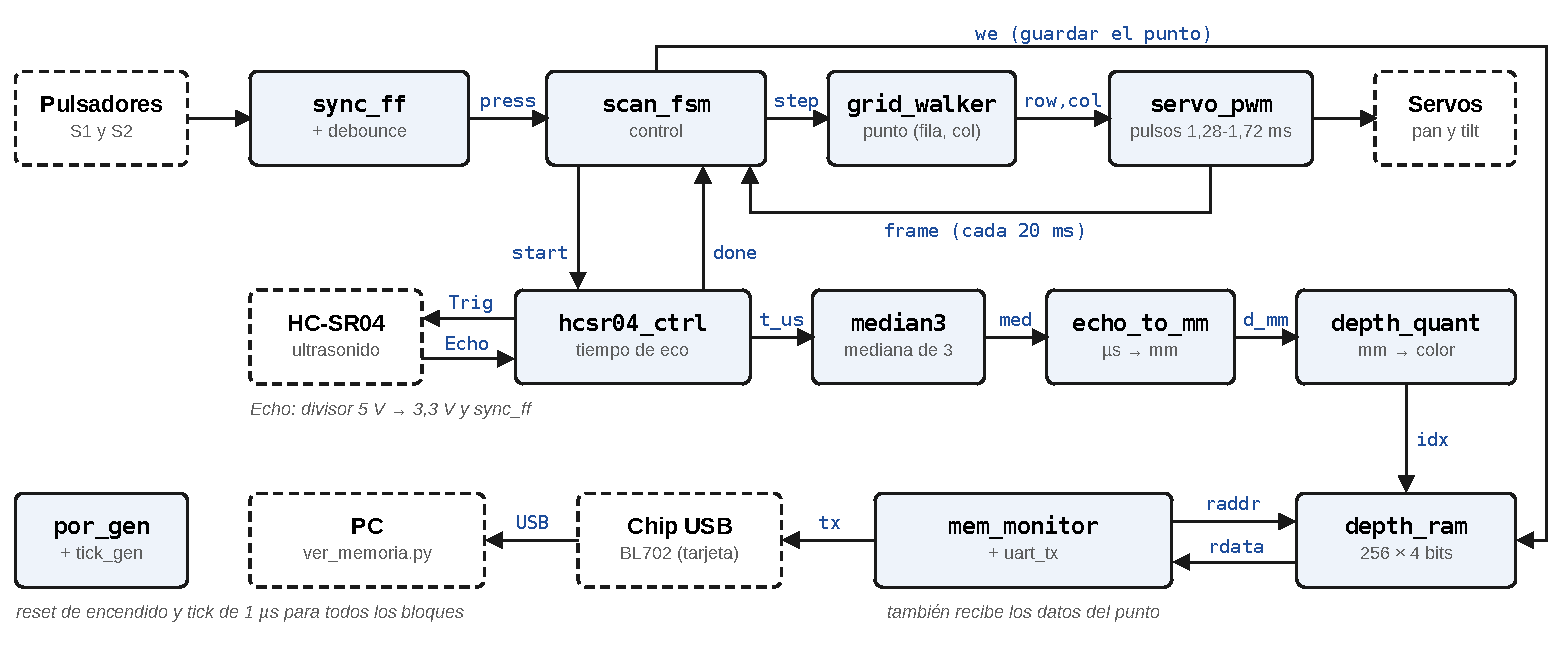
\includegraphics[width=\textwidth]{figuras/bloques.pdf}
\caption{Diagrama de bloques del sistema. Los bloques de borde punteado están fuera de la FPGA; las flechas muestran las señales principales entre componentes.}
\label{fig:bloques}
\end{figure*}

\subsection{Recorrido de un punto}
El funcionamiento se entiende siguiendo lo que pasa con un solo punto de la rejilla:
\begin{enumerate}
\item \mo{scan\_fsm} ordena un disparo (\mo{start}). \mo{hcsr04\_ctrl} genera el pulso Trig del sensor y mide, en microsegundos, cuánto dura en alto su salida Echo.
\item Lo anterior se repite tres veces, con una espera de al menos 60\,ms entre disparos para que el eco de un disparo no se confunda con el siguiente.
\item \mo{median3} se queda con la mediana de las tres mediciones, \mo{echo\_to\_mm} la convierte en milímetros y \mo{depth\_quant} en un índice de color de 4 bits.
\item \mo{scan\_fsm} escribe el índice en \mo{depth\_ram} (\mo{we}) en la dirección \{fila, columna\} y da la orden de avanzar (\mo{step}). \mo{grid\_walker} pasa al siguiente punto y \mo{servo\_pwm} mueve los servos durante la siguiente espera.
\item \mo{mem\_monitor} detecta la escritura, lee la memoria completa y la envía al computador por medio de \mo{uart\_tx}.
\end{enumerate}

\subsection{Un solo reloj}
Todo el sistema funciona con el oscilador de 27\,MHz de la tarjeta y es completamente síncrono: todos los registros cambian en el flanco de subida del mismo reloj. Las acciones que deben ocurrir más despacio no usan relojes más lentos, sino pulsos de habilitación de un ciclo de duración: \mo{tick} cada 1\us\ y \mo{frame} cada 20\,ms. Así no existen cruces entre dominios de reloj, y los únicos puntos donde una señal no respeta el reloj son las entradas externas, que pasan por \mo{sync\_ff}.

\subsection{Red de reset}
Existen dos señales de reset síncrono:
\begin{itemize}
\item \mo{rst\_btn = rst\_por}: solo el reset de encendido. Llega a \mo{tick\_gen}, \mo{sync\_ff} y \mo{debounce}.
\item \mo{rst = rst\_por + pressed\_S2}: el reset de encendido o el pulsador S2. Llega al resto del sistema.
\end{itemize}
La separación es necesaria porque el propio pulsador S2 depende de \mo{tick\_gen}, \mo{sync\_ff} y \mo{debounce}. Si S2 los reiniciara, el antirrebote de S2 quedaría congelado con \mo{pressed\_S2 = 1} y el sistema permanecería en reset para siempre.

\subsection{Metodología de diseño}
Cada componente se desarrolló con el mismo flujo:
\begin{enumerate}
\item Definir su función, su interfaz, el ancho de cada señal y sus casos límite.
\item Diseñar el circuito con los bloques del curso~\cite{harris} y dibujar su diagrama (anexos). Se buscó usar un único reloj y evitar multiplicadores y divisores.
\item Describirlo en Verilog siguiendo el diagrama.
\item Verificarlo con un testbench en Icarus Verilog~\cite{icarus} que revisa automáticamente sus casos límite.
\item Integrarlo en el módulo superior, sintetizarlo con Gowin EDA y comprobarlo en la tarjeta con el osciloscopio.
\end{enumerate}
La integración se hizo por etapas: primero el movimiento de los servos, después la cadena de medición y por último el envío al computador.

% =====================================================================
\section{Componentes del diseño}
% =====================================================================

Para cada componente se explica por qué es necesario, qué función cumple y las decisiones de diseño más importantes. El circuito de cada uno, construido con sumadores, comparadores, multiplexores, registros y máquinas de estados, se encuentra en los anexos.



% ---------------------------------------------------------------------
\subsection{Arranque y base de tiempo}

\subsubsection{\mo{por\_gen} (reset de encendido)}
\emph{Necesidad:} al encender, todos los registros deben empezar en un estado conocido, y algún circuito debe generar ese primer reset.
\emph{Función:} es un contador de 16 bits que, mientras no ha llegado a 1111\ldots1, mantiene \mo{rst\_por = 1}. Esto dura 65\,535 ciclos, es decir, 2,43\,ms. Al llegar a ese valor se detiene (su habilitación es \mo{listo'}), de modo que el reset nunca vuelve a activarse.
\emph{Decisión importante:} es el único registro del diseño sin entrada de reset, porque es el que lo genera. Parte de 0 gracias a que la FPGA pone todos sus flip-flops en su valor inicial al terminar de configurarse. La señal \mo{listo} enciende un LED.

\subsubsection{\mo{tick\_gen} (base de 1\us)}
\emph{Necesidad:} los tiempos del sistema (Trig, duración del eco, ancho de los pulsos de los servos y antirrebote) se expresan en microsegundos. Contarlos directamente en ciclos de 37\,ns exigiría contadores más anchos en cada componente.
\emph{Función:} un contador de 5 bits cuenta de 0 a 26 y entrega \mo{tick}, un pulso de un ciclo cada 27 ciclos, es decir, cada 1\us.
\emph{Decisión importante:} \mo{tick} no es un reloj sino una habilitación. Los contadores que miden microsegundos usan \mo{EN = tick} y siguen funcionando con el reloj de 27\,MHz.

\emph{¿Por qué trabajar en microsegundos?} Todas las especificaciones externas están dadas en microsegundos: el Trig debe durar al menos 10\us, Echo dura hasta 38\,000\us\ y los servos usan pulsos de 1280 a 1720\us\ dentro de periodos de 20\,000\us. Contar esos tiempos directamente en ciclos de 37\,ns exigiría contadores más anchos y constantes poco claras:
\begin{itemize}
\item 20\,ms son 540\,000 ciclos (20 bits), pero solo 20\,000\us\ (15 bits).
\item 5\,ms de eco son 135\,000 ciclos (18 bits), pero solo 5000\us\ (13 bits).
\end{itemize}
Con un único contador de 5 bits compartido, cada componente ahorra varios bits, las constantes del diseño son los mismos números de las hojas de datos y la conversión a milímetros usa un factor sencillo. La resolución de 1\us\ equivale a 0,17\,mm de distancia, muy por debajo de los 32\,mm que separan dos colores, así que no se pierde precisión útil.

% ---------------------------------------------------------------------
\subsection{Entradas externas}

\subsubsection{\mo{sync\_ff} (sincronizador)}
\emph{Necesidad:} los pulsadores y la señal Echo pueden cambiar en cualquier instante, sin respetar el reloj. Si una de ellas cambia justo en un flanco, el flip-flop que la captura puede quedar metaestable, y si la señal llega a varios registros, cada uno podría ver un valor distinto.
\emph{Función:} es un flip-flop que copia la entrada en cada flanco. A partir de él, la señal solo cambia justo después de un flanco, como todas las demás.
\emph{¿Por qué un solo flip-flop?} La solución habitual usa dos flip-flops en cadena: si el primero queda metaestable, tiene un ciclo completo para estabilizarse antes de que el segundo lo copie. En este diseño ese tiempo ya existe con uno solo. La salida de \mo{sync\_ff} pasa por muy pocas compuertas antes de llegar al siguiente registro, así que de los 37\,ns del periodo de 27\,MHz queda casi todo disponible para que una posible metaestabilidad se resuelva, y un flip-flop de la FPGA la resuelve en mucho menos tiempo. Además, estas señales cambian pocas veces por segundo (una pulsación, o un eco cada 60 a 80\,ms), lo que hace muy improbable que un cambio coincida exactamente con un flanco. Un segundo flip-flop solo agregaría un ciclo de retardo sin una mejora apreciable.

\emph{Otras decisiones:} el valor de reset es 1 para los pulsadores, que son activos en bajo, y 0 para Echo. Antes de llegar a la FPGA, Echo pasa por un divisor resistivo de 1\,k$\Omega$/2\,k$\Omega$ que reduce sus 5\,V a 3,3\,V.

\subsubsection{\mo{debounce} (antirrebote)}
\emph{Necesidad:} al presionar un pulsador mecánico, el contacto rebota durante algunos milisegundos. Sin filtrarlo, una sola pulsación de S1 se vería como varias y el barrido arrancaría y se detendría varias veces seguidas.
\emph{Función:} un cambio del pulsador solo se acepta si se mantiene durante 20\,ms (20\,000 ticks) seguidos. Si el pulsador rebota antes, el contador vuelve a cero. Entrega \mo{pressed}, que indica si el botón está presionado, y \mo{press}, un pulso de un ciclo en el momento de presionarlo.
\emph{Uso en el sistema:} S1 usa \mo{press} para iniciar o detener el barrido. S2 usa \mo{pressed} para mantener el reset mientras esté presionado.

% ---------------------------------------------------------------------
\subsection{Posicionamiento}

\subsubsection{\mo{grid\_walker} (recorrido de la rejilla)}
\emph{Necesidad:} el sistema debe saber en qué punto de la rejilla está y cuál es el siguiente.
\emph{Función:} guarda la fila y la columna actuales (4 bits cada una) y con cada pulso \mo{step} avanza un punto en serpentina: las filas pares se recorren de izquierda a derecha y las impares de derecha a izquierda. En el último punto, (11,\,0), activa \mo{last}, y el siguiente \mo{step} lo devuelve a (0,\,0).
\emph{Decisiones importantes:} con la serpentina el servo horizontal nunca hace el salto largo de un extremo al otro al cambiar de fila; ese salto solo ocurre una vez por imagen. Además entrega la dirección de memoria \mo{addr = \{row, col\}}, que se obtiene uniendo cables, sin multiplicar.

\subsubsection{\mo{servo\_pwm} (señales de los servos)}
\emph{Necesidad:} el SG90 recibe su posición como el ancho de un pulso que se repite cada 20\,ms.
\emph{Función:} un contador de periodo compartido cuenta de 0 a 19\,999\us. Cada canal mantiene su salida en 1 mientras el contador sea menor que el ancho $w$ del punto actual; esa comparación se hace con un restador.

\emph{Cálculo del ancho de pulso:} el SG90~\cite{sg90} está en su centro con un pulso de 1500\us\ y gira aproximadamente $1^\circ$ por cada 11\us. La ventana de observación debe cubrir el ancho del volumen de trabajo, 50\,cm, a su profundidad máxima, 70\,cm:
\begin{equation}
\theta = 2\arctan\!\left(\frac{25\ \text{cm}}{70\ \text{cm}}\right) \approx 39^\circ \;\rightarrow\; 40^\circ .
\end{equation}
Con 12 puntos por eje hay 11 pasos de $40^\circ/11 \approx 3{,}6^\circ$, es decir, unos $3{,}6 \cdot 11 \approx 40$\us\ por paso. La ventana ocupa $11 \cdot 40 = 440$\us\ y se centra en 1500\us, así que va de $1500 - 220 = 1280$\us\ a $1500 + 220 = 1720$\us:
\begin{equation}
w = 1280 + 40\cdot \mathit{idx}\ \ [\mu\text{s}], \qquad \mathit{idx} = 0,\ldots,11 .
\end{equation}
El producto se calcula sin multiplicador, como $40\cdot\mathit{idx} = 32\cdot\mathit{idx} + 8\cdot\mathit{idx}$: dos desplazamientos (5 y 3 posiciones, que son solo cables) y un sumador. Otro sumador agrega la base de 1280.
\emph{Decisiones importantes:} el ancho nuevo solo se carga al empezar un periodo, de modo que nunca se deforma un pulso en curso, y la salida pasa por un flip-flop para que no salgan glitches al pin. Además, al empezar cada periodo el componente genera \mo{frame}, que \mo{scan\_fsm} usa como base de tiempo de 20\,ms para todas sus esperas. Así no hace falta un temporizador adicional.

% ---------------------------------------------------------------------
\subsection{Medición}

\subsubsection{\mo{hcsr04\_ctrl} (control del sensor)}
\emph{Necesidad:} el HC-SR04 no entrega la distancia directamente. Hay que darle un pulso Trig y medir cuánto dura en alto su salida Echo, que es el tiempo de ida y vuelta del sonido.
\emph{Función:} una máquina de estados de cinco estados (IDLE, TRIG, WAIT\_RISE, MEASURE y WAIT\_FALL) junto con un contador de microsegundos. Con \mo{start} genera un Trig de 12\us\ (el sensor exige al menos 10\us~\cite{hcsr04}), espera a que Echo suba, cuenta los microsegundos que permanece en alto y entrega el resultado \mo{t\_us} con el pulso \mo{done}.
\emph{Decisiones importantes:} cada espera tiene un límite, para que el sistema nunca se quede bloqueado.
\begin{itemize}
\item Echo debe subir antes de 5000\us\ (\mo{RISE\_MAX}). El sensor utilizado tarda unos 2,2\,ms en responder.
\item La medición se satura en \mo{T\_MAX} = 5000\us, que equivale a unos 857\,mm, más que la profundidad del volumen de trabajo.
\item Cuando no hay eco, el sensor deja Echo en alto unos 38\,ms. Por eso \mo{done} solo se entrega cuando Echo ya bajó (como máximo 40\,ms, \mo{FALL\_MAX}). Así el siguiente disparo nunca encuentra al sensor ocupado.
\end{itemize}

\subsubsection{\mo{median3} (filtro de mediana)}
\emph{Necesidad:} el ultrasonido produce mediciones erróneas ocasionales, por ejemplo un eco que rebota en otra superficie o un eco perdido.
\emph{Función:} un registro de desplazamiento guarda las tres últimas mediciones. Tres comparadores, construidos con restadores, determinan cuál de ellas está en el medio, y un multiplexor la entrega.
\emph{¿Por qué la mediana?} Los errores del ultrasonido no son pequeñas variaciones alrededor del valor real, sino valores muy lejanos: un eco perdido, por ejemplo, se satura en 5000\us. Si un objeto a unos 300\,mm da las mediciones 1749, 1760 y 5000\us:
\begin{itemize}
\item el promedio es 2836\us, que equivale a 487\,mm y al color 8, un error de casi 19\,cm;
\item la mediana es 1760\us, que equivale a 302\,mm y al color 3, el correcto.
\end{itemize}
La mediana ignora por completo un valor extremo, mientras que el promedio lo reparte entre todos. Se usan tres mediciones porque es el menor número impar que permite descartar un error. Cada medición adicional costaría unos 80\,ms por punto, es decir, unos 11\,s más por imagen, y se superaría el límite de 40\,s.

\subsubsection{\mo{echo\_to\_mm} (conversión a milímetros)}
\emph{Necesidad:} la escala de colores se define en distancia, no en tiempo.
\emph{Origen de la ecuación:} el sonido viaja en el aire a $v \approx 343$\,m/s (a unos $20^\circ$C). El pulso Echo dura lo que tarda el sonido en llegar al objeto y regresar, es decir, en recorrer dos veces la distancia $d$. Por eso:
\begin{equation}
2d = v\,t \;\Rightarrow\; d = \frac{v\,t}{2}.
\end{equation}
Como $343$\,m/s $= 0{,}343$\,mm/$\mu$s, con $t$ en microsegundos:
\begin{equation}
d = \frac{0{,}343}{2}\,t = 0{,}1715\,t \ \ [\text{mm}].
\end{equation}
\emph{Función:} calcula esa distancia con un circuito combinacional, sin reloj.
\emph{Decisión importante:} para no multiplicar por un decimal, el factor se reemplaza por una fracción cuyo denominador es una potencia de 2. Como $0{,}1715 \cdot 64 = 10{,}98 \approx 11$:
\begin{equation}
d \approx \frac{11\,t}{64}, \qquad \frac{11}{64} = 0{,}171875 \ (+0{,}22\ \text{\%}).
\end{equation}
A 600\,mm ese error es de apenas 1,3\,mm, despreciable frente a los 32\,mm de cada color. El producto $11t = 8t + 2t + t$ se obtiene con dos desplazamientos (que son solo cables) y dos sumadores, y la división entre 64 consiste en descartar los 6 bits menos significativos. No se necesitan multiplicadores ni divisores. Como $t \leq 5000$ (\mo{T\_MAX}), $11t \leq 55\,000$ cabe en 16 bits.

\subsubsection{\mo{depth\_quant} (distancia a color)}
\emph{Necesidad:} la imagen tiene 16 colores, así que cada distancia debe convertirse en un índice de 4 bits.
\emph{Origen de la ecuación:} la escala debe cubrir la profundidad del volumen de trabajo, unos 70\,cm, con 15 colores, porque el color 16 se reserva para el fondo. Se empieza en 200\,mm porque los objetos de interés se ubican entre 20 y 70\,cm del sensor, y dedicar colores a distancias menores reduciría la resolución donde sí hay objetos. El paso se eligió como potencia de 2 para poder dividir sin un divisor: con 32\,mm por color, los 15 colores llegan hasta $200 + 15 \cdot 32 = 680$\,mm, prácticamente los 70\,cm del volumen. Así:
\begin{equation}
\mathit{idx} =
\begin{cases}
0, & d < 200\ \text{mm}\\[2pt]
\left\lfloor \dfrac{d - 200}{32} \right\rfloor, & 200 \leq d < 680\ \text{mm}\\[8pt]
15\ \text{(fondo)}, & d \geq 680\ \text{mm}
\end{cases}
\end{equation}
\emph{Función:} la resta $d - 200$ se hace con un sumador (el número 200 se suma en complemento a 2). Su acarreo de salida indica si $d \geq 200$. La división entre $32 = 2^5$ consiste en descartar los 5 bits menos significativos. Si el cociente pasa de 14, el índice se satura en 15.
\emph{Decisiones importantes:} la paleta (Tabla~\ref{tab:paleta}) recorre el espectro de rojo (cerca) a morado (lejos) en pasos de $20^\circ$ de tono, y el índice 15 es negro. Con esta escala, un objeto a 30\,cm toma el color 3 (amarillo) y uno a 60\,cm el color 12 (azul), así que se cumple el requisito de distinguirlos.

\begin{table}[t]
\centering
\caption{Paleta de colores de la imagen}
\label{tab:paleta}
\setlength{\tabcolsep}{3.5pt}
\begin{tabular}{@{}c l c c l c@{}}
\toprule
Índice & Distancia (mm) & Color & Índice & Distancia (mm) & Color \\
\midrule
0 & $<$ 232     & \sw{FF0000} & 8  & 456--487 & \sw{00FFAA} \\
1 & 232--263    & \sw{FF5500} & 9  & 488--519 & \sw{00FFFF} \\
2 & 264--295    & \sw{FFAA00} & 10 & 520--551 & \sw{00AAFF} \\
3 & 296--327    & \sw{FFFF00} & 11 & 552--583 & \sw{0055FF} \\
4 & 328--359    & \sw{AAFF00} & 12 & 584--615 & \sw{0000FF} \\
5 & 360--391    & \sw{55FF00} & 13 & 616--647 & \sw{5500FF} \\
6 & 392--423    & \sw{00FF00} & 14 & 648--679 & \sw{AA00FF} \\
7 & 424--455    & \sw{00FF55} & 15 & $\geq$ 680 (fondo) & \sw{000000} \\
\bottomrule
\end{tabular}
\end{table}

% ---------------------------------------------------------------------
\subsection{Almacenamiento: \mo{depth\_ram}}
\emph{Necesidad:} la imagen completa (144 puntos de 4 bits) debe guardarse mientras se construye, y debe poder leerse para enviarla al computador.
\emph{Función:} es una memoria de 256 palabras de 4 bits con dos puertos independientes. Por el puerto de escritura entra el color de cada punto medido, y por el de lectura \mo{mem\_monitor} lee su contenido.
\emph{Decisiones importantes:}
\begin{itemize}
\item La dirección es \{fila, columna\}. Así se evita calcular $\text{fila}\cdot 12 + \text{columna}$, que necesitaría un multiplicador, a cambio de dejar 112 palabras sin usar.
\item La lectura es registrada, es decir, el dato aparece un ciclo después de pedir la dirección. Esto permite que la herramienta de síntesis use un bloque de memoria dedicado (BSRAM)~\cite{bsram} de la FPGA en lugar de lógica.
\item Todas las palabras arrancan en 15, de modo que los puntos que aún no se han medido se ven como fondo negro.
\end{itemize}

% ---------------------------------------------------------------------
\subsection{Control: \mo{scan\_fsm}}
\emph{Necesidad:} alguien debe decidir cuándo disparar, cuánto esperar, cuándo guardar, cuándo avanzar y cuándo regresar al inicio, además de responder al pulsador S1.
\emph{Función:} es una máquina de Moore de seis estados: IDLE, FIRE, WAIT\_ECHO, GAP, WRITE y RETURN. Un contador de disparos cuenta cuántas mediciones lleva el punto actual y un contador de \mo{frame} mide las esperas. En cada punto el ciclo es FIRE $\rightarrow$ WAIT\_ECHO $\rightarrow$ GAP, repetido tres veces, y luego WRITE, que dura un ciclo y activa \mo{we} y \mo{step} al mismo tiempo.
\emph{Decisiones importantes:}
\begin{itemize}
\item La espera GAP dura \mo{N} = 4 frames (al menos 60\,ms), el tiempo que recomienda el fabricante entre disparos~\cite{hcsr04}. La espera que sigue a WRITE sirve además para que el servo llegue al punto nuevo, así que mover el sensor no cuesta tiempo adicional.
\item En el último punto, en lugar de GAP se espera \mo{RET} = 10 frames (200\,ms), porque los servos deben recorrer toda la ventana para regresar a (0,\,0).
\item WRITE es un estado aparte porque la mediana de la tercera medición está disponible un ciclo después de su \mo{done}.
\item S1 detiene el barrido desde cualquier estado. Al reanudar se pasa primero por GAP y se repiten los tres disparos del punto.
\end{itemize}

% ---------------------------------------------------------------------
\begin{figure*}[t]
\centering
\begin{tabular}{@{}c c@{}}
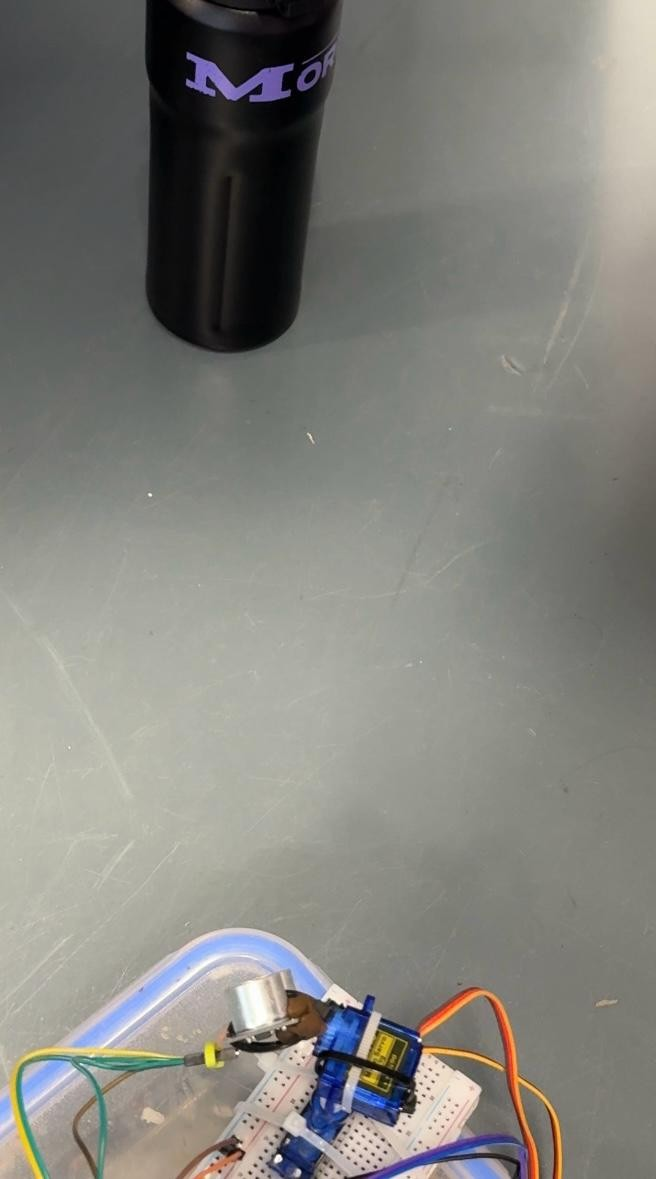
\includegraphics[height=5.4cm]{figuras/escena.jpg} &
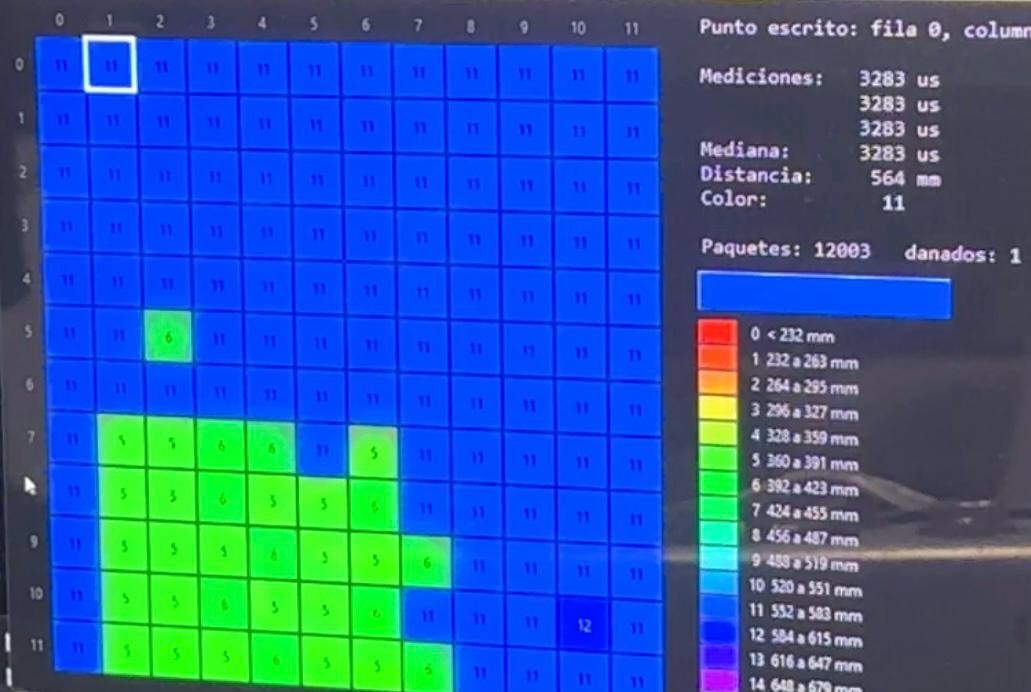
\includegraphics[height=5.4cm]{figuras/resultado.jpg} \\
(a) & (b)
\end{tabular}
\caption{(a) Escena de prueba: botella a unos 40\,cm, vista desde atrás del sensor. (b) Imagen obtenida en el computador: en cada casilla, el índice de color guardado en la memoria; a la derecha, los datos del último punto y la paleta.}
\label{fig:resultado}
\end{figure*}

\subsection{Envío al computador}

La Tang Nano 9K~\cite{tangnano} incluye, además de la FPGA, un chip BL702 que funciona como puente entre una línea serial y el USB, y que también se usa para programar la FPGA. El pin 17 de la FPGA está conectado a la entrada serial de ese chip, y en el computador aparece como un puerto COM. La FPGA solo tiene que generar la señal serial.

\subsubsection{\mo{uart\_tx} (transmisor serial)}
\emph{Necesidad:} solo hay un cable hacia el chip USB, así que los bits de cada carácter deben enviarse uno detrás de otro. Además, el computador no ve el reloj de la FPGA, por lo que ambos lados deben seguir un protocolo acordado.
\emph{Función:} usa el formato UART 8N1~\cite{chu}. La línea está en 1 mientras no se transmite. Cada byte se envía como un bit de inicio en 0, los 8 bits del dato empezando por el menos significativo y un bit de parada en 1. El bit de inicio le indica al receptor que debe empezar a contar el tiempo. Cada bit dura 234 ciclos, lo que da 115\,385 baudios (0,16\,\% sobre los 115\,200 nominales, dentro de la tolerancia del receptor). El circuito tiene un contador de ciclos por bit, un contador de bits restantes y un registro de desplazamiento de 10 bits cuya posición 0 es la salida.
\emph{Decisiones importantes:} en cada desplazamiento entra un 1, así que al terminar el registro queda lleno de unos y la línea vuelve sola al reposo. La salida sale directamente de un flip-flop, sin glitches. Una orden de envío que llegue mientras se transmite se ignora, y \mo{bdone} avisa cuando termina cada byte.

\subsubsection{\mo{mem\_monitor} (lectura y envío de la memoria)}
\emph{Necesidad:} el computador no puede ver el interior de la FPGA, así que la información de la imagen debe enviársele.
\emph{Función:} cada vez que se escribe un punto (\mo{we}), envía una línea de texto de 280 caracteres:
\begin{itemize}
\item la letra \texttt{P}, que marca el inicio;
\item 22 dígitos hexadecimales con la fila, la columna, el color, las tres mediciones, la mediana y la distancia;
\item los 256 dígitos de la memoria, leídos uno por uno por el puerto de lectura de \mo{depth\_ram};
\item un salto de línea, que marca el final.
\end{itemize}
La componen una máquina de Moore de cinco estados (IDLE, CHAR\_P, HEADER, DUMP y CHAR\_NL), un registro de cabecera de 88 bits que se desplaza 4 bits por cada dígito enviado y un contador que sirve como número de dígito en la cabecera y como dirección de la memoria. Cada dígito se convierte a código ASCII sumándole \texttt{0x30} si está entre 0 y 9, o \texttt{0x37} si está entre 10 y 15 (letras A a F).
\emph{Decisiones importantes:}
\begin{itemize}
\item Se lee la memoria real, de modo que lo que se ve en el computador es exactamente lo que está guardado. Si una línea se pierde, la siguiente trae otra vez la memoria completa.
\item Cada byte se envía dos ciclos después de cambiar la dirección, porque la memoria entrega el dato un ciclo más tarde.
\item Una línea tarda unos 24\,ms y entre dos puntos pasan unos 240\,ms, así que las líneas nunca se superponen.
\end{itemize}

\subsubsection{Programa del computador}
\mo{ver\_memoria.py} lee el puerto COM, comprueba que cada línea empiece con \texttt{P} y tenga 280 caracteres, y dibuja la rejilla de 12\,$\times$\,12 con la paleta de la Tabla~\ref{tab:paleta}, resaltando el último punto escrito y mostrando sus mediciones. Como la información es texto, también puede leerse en cualquier terminal serial.

% ---------------------------------------------------------------------
\subsection{Integración: \mo{lidar\_top\_monitor}}
Es el módulo superior. No tiene lógica propia de barrido: crea una copia de cada componente, une sus señales y forma la red de reset. Sus puertos son los pines de la Tabla~\ref{tab:pines}. Los seis LEDs de la tarjeta, que son activos en bajo, muestran si el barrido está activo (\mo{running}), si terminó el arranque (\mo{listo}) y, en los cuatro restantes, el índice de color de la última medición, lo que permite comprobar el sensor sin el computador.

% =====================================================================
\section{Montaje experimental}
% =====================================================================

\subsection{Equipos}
\begin{itemize}
\item \textbf{Tarjeta Tang Nano 9K}~\cite{tangnano}: FPGA GW1NR-9~\cite{gw1nr}, oscilador de 27\,MHz y chip BL702 como puente USB a serial. Un solo cable USB alimenta la tarjeta, la programa y lleva los datos al computador.
\item \textbf{Sensor HC-SR04}~\cite{hcsr04} (un clon que tarda unos 2,2\,ms en responder al Trig), alimentado a 5\,V. Su salida Echo llega a la FPGA a través de un divisor resistivo de 1\,k$\Omega$/2\,k$\Omega$.
\item \textbf{Dos servomotores SG90}~\cite{sg90} montados como soporte \emph{pan-tilt} sobre una protoboard, con el sensor en el servo vertical.
\item \textbf{Fuente externa de 5\,V} para los servos y el sensor, con la tierra unida a la de la tarjeta.
\item \textbf{Computador} con el programa \mo{ver\_memoria.py} (Python), que lee el puerto COM y dibuja la imagen.
\item \textbf{Osciloscopio} para comprobar las señales Trig, Echo y las de los servos.
\end{itemize}
La síntesis, la ubicación y la programación se hicieron con Gowin EDA, y la simulación con Icarus Verilog~\cite{icarus}. La Tabla~\ref{tab:pines} muestra los pines usados.

\begin{table}[t]
\centering
\caption{Pines de la tarjeta utilizados}
\label{tab:pines}
\begin{tabular}{@{}l c l@{}}
\toprule
Señal & Pin & Conexión \\
\midrule
\mo{clk\_27}   & 52 & Oscilador de 27\,MHz de la tarjeta \\
\mo{btn\_s1}   & 4  & Pulsador S1: iniciar / detener \\
\mo{btn\_s2}   & 3  & Pulsador S2: reset del sistema \\
\mo{pwm\_pan}  & 25 & Señal del servo horizontal \\
\mo{pwm\_tilt} & 26 & Señal del servo vertical \\
\mo{trig}      & 27 & Trig del HC-SR04 \\
\mo{echo}      & 28 & Echo del HC-SR04 (divisor 1\,k$\Omega$/2\,k$\Omega$) \\
\mo{tx\_pc}    & 17 & Línea serial hacia el chip USB \\
\mo{led[5:0]}  & 10--16 & LEDs de la tarjeta \\
\bottomrule
\end{tabular}
\end{table}

\subsection{Escena de prueba}
Como fondo se usó una superficie plana, ubicada en diagonal de modo que la distancia recta del sensor a cada punto fuera aproximadamente la misma. Frente a ella se colocó una botella a unos 40\,cm del sensor (Fig.~\ref{fig:resultado}a).

% =====================================================================
\section{Resultados experimentales}
% =====================================================================



\subsection{Señales}
Con el osciloscopio se comprobó que el Trig dura 11\us\ y se repite cada unos 80\,ms, y que el ancho de Echo cambia con la distancia del objeto. Las señales de los servos tienen un periodo de 20\,ms y un ancho que cambia de un punto a otro entre 1,28 y 1,72\,ms, como se diseñó.

\subsection{Imagen de profundidad}
La Fig.~\ref{fig:resultado}b muestra la imagen obtenida:
\begin{itemize}
\item \textbf{Fondo:} casi todos los puntos tienen el color 11 (552 a 583\,mm). Por ejemplo, el último punto medido dio 3283\us, es decir, 564\,mm. El color es uniforme, como se esperaba con el fondo en diagonal.
\item \textbf{Botella:} aparece como una región de colores 5 y 6 (360 a 423\,mm), que corresponde a los 40\,cm a los que se ubicó. Se distingue claramente del fondo, separada por 5 o 6 colores (unos 16 a 20\,cm).
\item \textbf{Tamaño de la botella:} la región es más ancha que la botella. El haz del HC-SR04 tiene una apertura de unos $15^\circ$~\cite{hcsr04}, que a 40\,cm cubre un círculo de unos 10\,cm de diámetro, mientras que entre dos puntos vecinos hay $3{,}6^\circ$ (unos 2,5\,cm). Por eso varios puntos vecinos ven la botella dentro de su haz y miden su distancia, que es la más cercana.
\item \textbf{Puntos aislados:} dos puntos, (5,\,2) y (10,\,10), tienen un color distinto al de sus vecinos. Son mediciones erróneas en las que dos de los tres disparos fallaron, caso que la mediana no puede corregir.
\end{itemize}

\subsection{Tiempo por imagen y enlace serial}
Recorrer una fila de 12 puntos tomó 2,85\,s, es decir, unos 0,24\,s por punto. Este tiempo está dominado por las tres esperas de 60 a 80\,ms de cada punto. Los 144 puntos toman unos 34\,s, más 0,2\,s de regreso, por debajo del límite de 40\,s. En el computador se recibieron 12\,003 líneas y solo una se descartó por llegar incompleta.

% =====================================================================
\section{Conclusiones}
% =====================================================================

\begin{itemize}
\item Usar un único reloj de 27\,MHz y generar los tiempos lentos con pulsos de habilitación (\mo{tick} y \mo{frame}) evitó los problemas de cruzar dominios de reloj. Las únicas señales asíncronas, los pulsadores y Echo, se sincronizan a la entrada.
\item Elegir pasos que son potencias de 2 (11/64 para convertir a milímetros y 32\,mm por color) y direcciones formadas por concatenación permitió hacer todas las operaciones con sumadores, desplazamientos y selección de bits, sin multiplicadores ni divisores.
\item La mediana de tres disparos, junto con los límites de espera de \mo{hcsr04\_ctrl}, hace que el sistema tolere mediciones erróneas y ausencia de eco sin bloquearse.
\item Enviar la memoria completa por el puerto USB de la tarjeta, leyéndola por su propio puerto de lectura, permite observar en tiempo real cómo se llena la imagen y confirmar que los datos quedaron realmente guardados.
\item Se cumplen los requisitos: la imagen se obtiene en unos 34\,s; por diseño, los objetos a 30 y 60\,cm toman los colores 3 y 12, y en la prueba una botella a 40\,cm se distinguió de un fondo a 56\,cm por 5 a 6 colores.
\item La resolución lateral está limitada por la apertura del haz del sensor, que es más ancha que el paso entre puntos: los objetos aparecen más anchos de lo que son.
\end{itemize}

\begin{thebibliography}{8}
\bibitem{harris} D. M. Harris y S. L. Harris, \emph{Digital Design and Computer Architecture}, 2.ª ed. Waltham, MA, EE.~UU.: Morgan Kaufmann, 2012.
\bibitem{hcsr04} ElecFreaks, ``Ultrasonic Ranging Module HC-SR04,'' hoja de datos.
\bibitem{sg90} Tower Pro, ``SG90 Micro Servo,'' hoja de datos.
\bibitem{tangnano} Sipeed, ``Tang Nano 9K,'' documentación de la tarjeta. [En línea]. Disponible: https://wiki.sipeed.com
\bibitem{gw1nr} GOWIN Semiconductor, ``GW1NR Series of FPGA Products,'' hoja de datos.
\bibitem{bsram} GOWIN Semiconductor, ``Gowin BSRAM \& SSRAM User Guide,'' guía de usuario.
\bibitem{chu} P. P. Chu, \emph{FPGA Prototyping by Verilog Examples}. Hoboken, NJ, EE.~UU.: Wiley, 2008.
\bibitem{icarus} S. Williams, ``Icarus Verilog.'' [En línea]. Disponible: https://steveicarus.github.io/iverilog/
\end{thebibliography}

% =====================================================================
% ANEXOS
% =====================================================================
\clearpage
\onecolumn
\renewcommand{\thefigure}{A\arabic{figure}}
\setcounter{figure}{0}

\begin{landscape}
\section*{Anexos: diagramas de cada componente}

En los diagramas se usan los símbolos del curso: la marca diagonal sobre un cable indica su número de bits, las etiquetas con el mismo nombre representan el mismo cable y las constantes se escriben en binario.

\newcommand{\anexo}[3][0.85]{%
\begin{center}
\includegraphics[width=\textwidth,height=#1\textheight,keepaspectratio]{figuras/#2.pdf}
\captionof{figure}{#3}
\end{center}
\clearpage}

\anexo[0.72]{lidar_top_monitor}{Módulo superior \mo{lidar\_top\_monitor}: conexión de todos los componentes.}
\anexo{por_gen}{\mo{por\_gen}: reset de encendido.}
\anexo{tick_gen}{\mo{tick\_gen}: base de tiempo de 1\us.}
\anexo{sync_ff}{\mo{sync\_ff}: sincronizador de entradas externas.}
\anexo{debounce}{\mo{debounce}: antirrebote de los pulsadores.}
\anexo{grid_walker}{\mo{grid\_walker}: recorrido en serpentina de la rejilla.}
\anexo{servo_pwm}{\mo{servo\_pwm}: señales de los servos y pulso \mo{frame}.}
\anexo{hcsr04_ctrl}{\mo{hcsr04\_ctrl}: circuito del control del sensor.}
\anexo{hcsr04_ctrl_estados}{\mo{hcsr04\_ctrl}: diagrama de estados.}
\anexo{median3}{\mo{median3}: filtro de mediana de tres mediciones.}
\anexo{echo_to_mm}{\mo{echo\_to\_mm}: conversión de tiempo de eco a milímetros.}
\anexo{depth_quant}{\mo{depth\_quant}: conversión de distancia a índice de color.}
\anexo{paleta}{Paleta de 16 colores.}
\anexo{depth_ram}{\mo{depth\_ram}: memoria de la imagen.}
\anexo{scan_fsm_final}{\mo{scan\_fsm}: circuito de la máquina de control.}
\anexo{scan_fsm_estados}{\mo{scan\_fsm}: diagrama de estados.}
\anexo{uart_tx}{\mo{uart\_tx}: transmisor serial UART 8N1.}
\anexo{mem_monitor}{\mo{mem\_monitor}: circuito de lectura y envío de la memoria.}
\anexo{mem_monitor_estados}{\mo{mem\_monitor}: diagrama de estados.}

\end{landscape}
\end{document}
